\section{SECH 5}
\subsection{Motivations and Deployment Scenarios}

[ ] arbitrary access for new clients without coordination from server

\subsection{Design}

A server produces an \var{SECHConfig} which specifies a \ac{HPKE} cipher suite
(\ac{KEM}, \ac{HKDF}, and \ac{AEAD} IDs),
a public key for the \ac{KEM}, and the server
also maintains the corresponding private key for the public key.
For simplicity in this specification we assert that the \ac{HKDF}
and \ac{AEAD} are chosen at \var{SECHConfig}-compilation time.
This is unlike \ac{ECH} where the \ac{HKDF} and \ac{AEAD} are
negotiated for each session.

A client has to securely obtain the \var{SECHConfig} in order to offer \ac{SECH} 5 in a \var{ClientHello}, e.g. using \ac{DoH} or by any other secure and confidential means.

The client first produces the \var{ClientHello} as would be done normally
for \ac{TLS} 1.3 up to the point of computing the \ac{PSK} \var{binder}.

The client instantiates a \ac{HPKE} context using the suite specified in
the \var{SECHConfig} and produces a 32 octet \var{enc}.
As of writing the only \ac{KEM} with a 32 octet \var{enc} in the \ac{IANA} is
the \ac{X25519} \ac{EC}.
The \var{enc} is produced by generating a 32 octet random key, $k$, and then encrypting
that key with the public key from the \var{SECHConfig}.
The \var{random} field is set to value of \var{enc}.

The client concatenates the inner servername and inner \ac{ALPN} list separated by null bytes, and pads this to 16 bytes with 0s. Call the resulting string \var{sech\_cleartext}.
The client creates \var{ClientHelloOuterAAD} which is a clone
of the \var{ClientHello} but with the \var{legacy\-\_session\-\_id} field set to 0s,
and the \var{binders} list truncated off.
Using the \ac{AEAD} specified in the \var{SECHConfig} the client encrypts
\var{sech\_cleartext} with \var{ClientHelloOuterADD} as \ac{AAD}
producing a 32 octet ciphertext \var{sech\_cipher}
(including the 16 byte \ac{AEAD} tag). 
For simplicity we assert in this draft that only \ac{AEAD}s with a 16 byte tag are valid in an \var{SECHConfig}.

% [ ] client encrypts the \var{padded\_servername} with the AEAD specified in SECHConfig, and with key $k$ and a \nonce which is the first 12 octets of the hash of \var{SECH5ClientHelloAAD}, and with \var{SECH5ClientHelloAAD} as AAD, producing \var{sech5\_cipher} which is the concatenation of the encrypted text and the tag $t$

% [ ] \var{SECH5ClientHelloAAD} is the \var{ClientHello} but with the portion in which the AEAD cipher (encrypted text and tag) will be placed set to zero, the size and location of this region depends on \var{SECHConfig}

% [ ] \var{SECH5ClientHelloAAD} is the \var{ClientHelloOuter} but with the \var{random} and \var{legacy\_session\_id} set to all 0s

The client encodes \var{enc} and \var{sech\_cipher} in the \var{ClientHello} \var{random} and \var{legacy\_session\_id} fields producing a partial \var{ClientHelloOuter}
(excluding the \var{binders})
as depicted in Figure~\ref{fig:sech5-cover}.
If the client is using a resumption \ac{PSK} controlled by the backend server
the \var{binders} list is computed
using the synthetic \var{ClientHelloInner} transcript rather
than the transcript of \var{ClientHelloOuter}.

The \var{ClientHelloInner} has the \var{random} field replaced with \varsechinnerrandom{}, and the first 16 bytes of the
\varlegacysessionid{} replaced with \var{sech\_clear}.
Also, the extension data field of the outer \ac{SNI} is set to all 0s.

The client-facing server attempts to decapsulate \var{enc} with the private key associated with \var{SECHConfig} retrieving $k$, on failure 
the client-facing server continues with normal TLS 1.3,
although implementations should ensure that the timing of the response in case of \ac{SECH}
decryption failure is not distinguishable from the case when
\ac{SECH} succeeds.
Using the \ac{HKDF} in \var{SECHConfig} $k$ is transformed into \varsechinnerrandom{}.

% [ ] TODO: Unlike \ac{ECH} we do not support arbitrary numbers \var{SECHConfig}s on the server
% in order to ensure the server response time is consistent and does not reveal \ac{SECH}
% decryption success or failure. 

The client-facing server computes \var{ClientHelloOuterAAD} and the \nonce, and then attempts to decrypt and retrieve \var{sech\_cleartext}, on failure  
the client-facing server continues with a normal TLS 1.3 handshake.

On success the client-facing server constructs \var{ClientHelloInner} by replacing 
the first 16 bytes of \var{ClientHelloOuter}'s \var{legacy\-\_session\-\_id}
with \var{sech\_clear}, and also replacing the \var{random} field
with $k$. Also the \var{extension\_data} of the \var{server\_name} extension is set to all 0s.

The client-facing server forwards \var{ClientHelloInner} to the backend server
(over a channel secured and authenticated by some other means).
The backend server processes this message, detecting the all-zero \ac{SNI} extension value,
and decodes the inner \ac{SNI} and \ac{ALPN} from the \varlegacysessionid{}.

If the backend server needs to negotiate different parameters by sending a
\var{HelloRetryRequest} this message is constructed as in normal \ac{TLS} 1.3.
The \var{HelloRetryRequest} message has no cover for a stealthy acceptance signal.

The subsequent \var{ClientHello2}'s \var{random} and \varlegacysessionid{} fields
must be identical to the first \var{ClientHello} so as not to stick out from normal
\ac{TLS} 1.3. This means the \var{ClientHello2} has no cover for hiding a second
\ac{SECH} payload, which means the \var{ClientHello2} is malleable and 
vulnerable to \var{HelloRetryRequest} hijacking.
Therefore, in the case of a \var{HRR} the remainder of the handshake is simply intended
to prevent revelation to the attacker that \ac{SECH} was attempted, and
the client and backend server give up on the connection.

To achieve this, when a client-facing server receives a \var{ClientHello2} it always
forwards it to the backend server corresponding to the outer \ac{SNI} in the \var{ClientHello2}. Ideally this `cover' backend server should support a superset of
the parameters supported by all \ac{SECH} backend servers such that the \var{ClientHello2}
will be accepted by the `cover' backend.

In the case that no \var{HRR} is triggered the backend server can continue to signal
its acceptance of \ac{SECH}.
The \var{ServerHello} contains a special \var{sech\_accept\_confirmation} value in the last 8 octets of the \var{random} field.


\begin{figure}[htb]
\centering
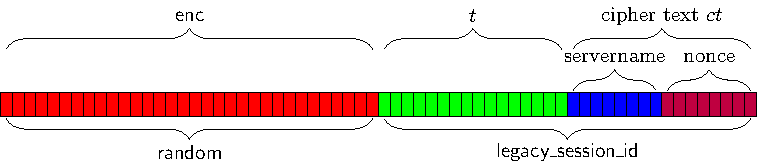
\includegraphics[width=\linewidth]{figure/sech5-cover.pdf}
\captionsetup{width=.8\linewidth} 
\caption[SECH 5 Cover]{}
\label{fig:sech5-cover}
\end{figure}

\subsection{Implementation Notes}